22. \begin{figure}[ht!]
\center{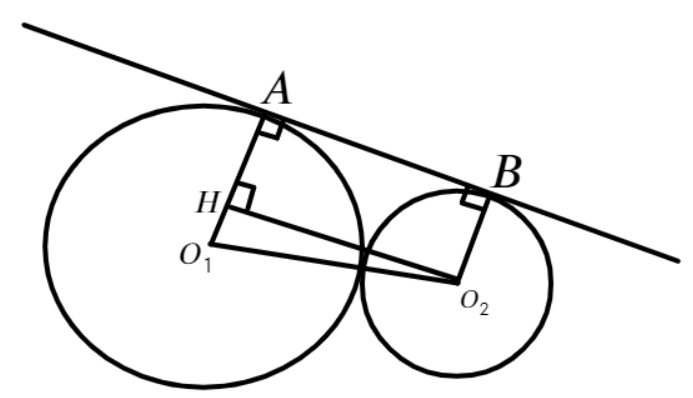
\includegraphics[scale=0.35]{g8-22.png}}
\end{figure}\\
Радиусы, проведённые к точке касания, перпендикулярны касательной, поэтому $O_1ABO_2$ является прямоугольной трапецией. Точка касания двух окружностей лежит на одной прямой с их центрами, поэтому $O_1O_2=8+2=10.$ Проведём высоту $O_2H,$ тогда $HABO_2$ является прямоугольником и $AH=O_2B=2,$ тогда $O_1H=O_1A-AH=8-2=6.$ По теореме Пифагора $O_2H=\sqrt{O_1O_2^2-O_1H^2}=\sqrt{10^2-6^2}=8,$ тогда $AB=O_2H=8.$\\
